\ifx\wholebook\relax \else

\documentclass[UTF8]{article}

\usepackage[nomarginpar
  %, margin=.5in
]{geometry}

\addtolength{\oddsidemargin}{-0.05in}
\addtolength{\evensidemargin}{-0.05in}
\addtolength{\textwidth}{0.1in}

\usepackage[cn]{../../prelude}

\setcounter{page}{1}

\begin{document}

\title{参考答案}

\author{刘新宇
\thanks{{\bfseries 刘新宇} \newline
  Email: liuxinyu95@gmail.com \newline}
  }

\maketitle
\fi

\markboth{参考答案}{编程中的数学}

\chapter*{参考答案}
\phantomsection  % so hyperref creates bookmarks
\addcontentsline{toc}{chapter}{参考答案}

\section{前言}

\begin{enumerate}
\item 编程实现一个井字棋游戏是传统人工智能中的经典问题,而计算机可以轻松算出三个数字的和并判断其是否等于15。请利用这个同构编写一个简化的井字棋程序,并做到不被人类玩家击败。

我们的思路是使用《洛书》幻方来同构井字棋游戏,我们用集合$X$, $O$来保存两个玩家所占领的格子。对于前言中的对局,开始时$X = \phi$,$O = \phi$,结束时$X = \{ 2, 5, 7, 1 \}$,$O = \{ 4, 3, 8, 6 \}$。为此我们需要先写一个程序判断一个集合中是否有3个元素相加等于15,从而知道某个玩家获胜与否。

有两种思路解决这个问题,第一种是列举洛书幻方中的所有行、列、对角线,共8个三元组:$\{ \{4, 9, 2\}, \{3, 5, 7\}, ..., \{2, 5, 8\} \}$。然后看是否某个三元组包含在玩家占领的格子集合中。第二种比较有趣,假设玩家占领了格子$ X = \{x_1, x_2, ..., x_n\}$。这些格子按照洛书幻方中的元素升序排列。我们可以先选出$x_1$,然后用左右两个指针$l, r$分别指向下一个元素和最后一个元素,然后把这3个数加起来$s = x_1 + x_l + x_r$,如果等于15,说明玩家连成一条直线已经获胜了。如果小于15,由于元素是升序排列的,我们可以把左侧指针$l$加一,然后再次尝试;如果大于15,我们把右侧指针$r$减一,然后再次尝试。如果左右指针相遇,说明固定$x_1$没有找到相加等于15的三元组,我们选出$x_2$再次进行这样的检查。这样最差情况总共进行$(n - 2)+ (n - 3) + ... + 1$次检查就得知玩家是否获胜了。

\lstset{language=Python
    , frame=single
}
\begin{lstlisting}
def win(s):
    n = len(s)
    if n < 3:
        return False
    s = sorted(s)
    for i in range(n - 2):
        l = i + 1
        r = n - 1
        while l < r:
            total = s[i] + s[l] + s[r]
            if total == 15:
                return True
            elif total < 15:
                l = l + 1
            else:
                r = r - 1
    return False
\end{lstlisting}

这样给定$X$和$O$,就能判断局面。如果$X$和$O$占满全部9个格子,还未分出胜负,则表示平局。接下来我们用传统人工智能中的$min-max$方法来实现井字棋,我们给每个局面一个评分,一方试图让评分最大化,称为正方;另一方试图让评分最小化,称为反方,从而实现对抗。平局的话评分为0,如果某个局面让正方获胜,我们设置评分为10,反方获胜评分为-10。这个分数值完全是随意设置的,不影响结果。

\begin{lstlisting}
WIN = 10
INF = 1000

# Luo Shu magic square
MAGIC_SQUARE = [4, 9, 2,
                3, 5, 7,
                8, 1, 6]

def eval(x, o):
    if win(x):
        return WIN
    if win(o):
        return -WIN
    return 0

def finished(x, o):
    return len(x) + len(o) == 9
\end{lstlisting}

对于任何一个对局,我们都让计算机不断向前探索,直到找到输赢或者平局的确定局面才停下来。探索的方法是穷尽当前所有能占领的格子,然后转换身份,考虑自己是对方时怎样对抗。对于所有候选方案,如果是正方,就选择评分高的方案,如果是反方,就选择评分低的方案。

\begin{lstlisting}
def findbest(x, o, maximize):
    best = -INF if maximize else INF
    move = 0
    for i in MAGIC_SQUARE:
        if (i not in x) and (i not in o):
            if maximize:
                val = minmax([i] + x, o, 0, not maximize)
                if val > best:
                    best = val
                    move = i
            else:
                val = minmax(x, [i] + o, 0, not maximize)
                if val < best:
                    best = val
                    move = i
    return move
\end{lstlisting}

$min-max$是一个递归搜索的过程,为了尽快获胜,我们在评分上加上对向前探索步数的考虑。如果是正方,就从评分中减去递归深度,而对于反方,则加上递归深度。

\begin{lstlisting}
def minmax(x, o, depth, maximize):
    score = eval(x, o)
    if score == WIN:
        return score - depth
    if score == -WIN:
        return score + depth
    if finished(x, o):
        return 0  # draw
    best = -INF if maximize else INF
    for i in MAGIC_SQUARE:
        if (i not in x) and (i not in o):
            if maximize:
                best = max(best, minmax([i] + x, o, depth + 1, not maximize))
            else:
                best = min(best, minmax(x, [i] + o, depth + 1, not maximize))
    return best
\end{lstlisting}

现在我们就做出一个无法被人类击败的程序了,我们的程序在背后用洛书幻方对抗人类玩家:

\begin{lstlisting}
def board(x, o):
    for r in range(3):
        print "-----------"
        for c in range(3):
            p = MAGIC_SQUARE[r*3 + c]
            if p in x:
                print "|X",
            elif p in o:
                print "|O",
            else:
                print "| ",
        print "|"
    print "-----------"

def play():
    x = []
    o = []
    while not (win(x) or win(o) or finished(x, o)):
        board(x, o)
        while True:
            i = int(input("[1..9]==>"))
            if i not in MAGIC_SQUARE or MAGIC_SQUARE[i-1] in x or
               MAGIC_SQUARE[i-1] in o:
                print "invalid move"
            else:
                x = [MAGIC_SQUARE[i-1]] + x
                break
        o = [findbest(x, o, False)] + o
    board(x, o)
\end{lstlisting}

\end{enumerate}

\section{自然数}

\begin{enumerate}
\item 定义0的后继为1,证明对于任何自然数都有$a \cdot 1 = a$

首先用数学归纳法证明$0 + a = a$这个结论,见附录I。然后:
\[
\begin{array}{rlr}
a' \cdot 1 & = a' \cdot 0' & \text{定义0的后继为1} \\
           & = a' \cdot 0 + a' & \text{乘法定义规则二} \\
           & = 0 + a' & \text{乘法定义规则一} \\
           & = a' & \text{此前证明的结论}
\end{array}
\]

\item 证明乘法分配律

可以用数学归纳法证明左侧的分配律$c(a + b) = ca + cb$。首先是$b = 0$的情况:

\bre
c(a + 0) & = & ca & \text{加法规则一} \\
         & = & ca + 0 & \text{反向用加法规则一} \\
         & = & ca + c0 & \text{反向用乘法规则一} \\
\ere

递推假设$c(a + b) = ca + cb$,接下来证明$c(a + b') = ca + cb'$

\bre
c(a + b') & = & c(a + b)' & \text{加法规则二} \\
          & = & c(a + b) + c & \text{乘法规则二} \\
          & = & ca + cb + c & \text{递推假设} \\
          & = & ca + (cb + c) & \text{加法结合律} \\
          & = & ca + cb' & \text{反向用乘法规则二} \\
\ere

\item 证明乘法结合律和交换律

我们只证明乘法结合律$(ab)c = a(bc)$,乘法交换律的证明则给出一个提纲。利用数学归纳法,首先是$c = 0$的情况:

\bre
(ab)0 & = & 0 & \text{乘法规则一} \\
      & = & a0 & \text{反向用乘法规则一} \\
      & = & a(b0) & \text{反向用乘法规则一} \\
\ere

递推假设$(ab)c = a(bc)$,接下来要证明$(ab)c' = a(bc')$

\bre
(ab)c' & = & (ab)c + ab & \text{乘法规则二} \\
       & = & a(bc) + ab & \text{递推假设} \\
       & = & a(bc + b) & \text{上题证明的分配律} \\
       & = & a(bc') & \text{反向用乘法规则二} \\
\ere

证明乘法交换律可以分为三步,都使用数学归纳法。首先证明$1a = a$,然后再证明右侧的分配律$(a + b)c = ac + bc$,最后再证明交换律。

\item 如何利用皮亚诺公里验证3 + 147 = 150

我们先看看经典的2 + 2 = 4是怎么证明的:

\bre
2 + 2 & = & 0'' + 0'' & \text{2是0的两次后继} \\
      & = & (0'' + 0')' & \text{加法定义规则二} \\
      & = & ((0'' + 0)')' & \text{加法定义规则二} \\
      & = & ((0'')')' & \text{加法定义规则一} \\
      & = & 0'''' = 4 & \text{0的4次后继} \\
\ere

显然用这个方法证明3 + 147 = 150的话太冗长了,我们可以用先前证明的加法交换律证明147 + 3 = 150会容易一些。另一个方法是通过数学归纳法证明$3 + a = a'''$。

\item 试给出乘法分配律,乘法结合律,和乘法交换律的几何解释。

\begin{figure}[htbp]
 \centering
 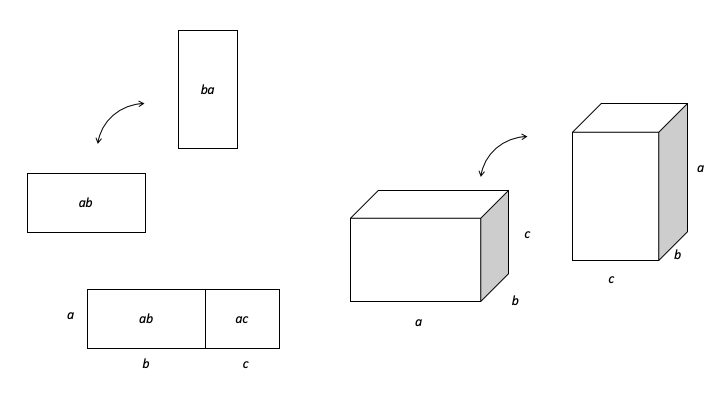
\includegraphics[scale=0.4]{img/geometric-arithmetic.png}
 \captionsetup{labelformat=empty}
 \caption{乘法交换律、结合律、分配律的几何解释}
 \label{fig:geometric-arithmetic}
\end{figure}


\item 使用$foldn$定义平方$()^2$。

可以利用递推关系$(n+1)^2 = n^2 + 2n + 1$来定义平方:

\[
()^2 = 2nd \cdot foldn\ (0, 0)\ h
\]

其中$h$接受一对值$(i, s)$,分别代表自然数$i$和它的平方$s$。它将第一个值递增1,然后利用平方展开式求出下一个平方数。

\[
h\ (i, s) = (i + 1, s + 2i + 1)
\]

\item 使用$foldn$定义$()^m$,计算给定自然数的$m$次幂。

一种简单的方法是借助第一章中定义的$m^{()} = foldn(1, (\cdot m))$来定义$()^m$:

\[
()^m = 2nd \cdot foldn\ (0, 0)\ h
\]

其中

\[
h\ (i, b) = (i + 1, (i + 1)^m)
\]

这看起来有些奇怪,所有中间计算都被直接丢掉了。另一种方法是利用牛顿二项式定理:

\[
(n + 1)^m = n^m + \binom{m}{1} n^{m-1} + ... + \binom{m}{m-1} n + 1
\]

这样就建立了递推关系:

\[
(n)^m = 2nd(foldn\ (1, 1)\ h\ (n - 1))
\]

其中

\[
h (i, x) = (i + 1, C \cdot X)
\]

这里$C \cdot X$是二项式系数和各次幂的点积$C \cdot X = \sum c_j x_j$。各次幂可以通过对$x$不断除以$i$求出,二项式定理的系数可以由帕斯卡三角形逐行递推得到。下面是综合在一起的例子程序:

\lstset{language=Haskell
    , frame=single
}
\begin{lstlisting}
exp m n = snd $ foldn (1, 1) h (n - 1) where
  cs = foldn [1] pascal m
  h (i, x) = (i + 1, sum $ zipWith (*) cs xs) where
    xs = take (m + 1) $ iterate (`div` i) x

pascal = gen [1] where
  gen cs (x:y:xs) = gen ((x + y) : cs) (y:xs)
  gen cs _ = 1 : cs
\end{lstlisting}

\item 使用$foldn$定义奇数的和。它会产生怎样的序列?

用$foldn$定义1 + 3 + 5 + ...为$2nd \cdot foldn\ (1, 0)\ h$,其中:

\[
h\ (i, s) = (i + 2, s + i)
\]

如第一章中习题下的插图所示,奇数和总是平方数。

\item 地面上有一排洞,一只狐狸藏在某个洞中。每天狐狸会移动到相邻的下一个洞里。如果每天只能检查一个洞,请给出一个捉到狐狸的策略,并证明这个策略有效。如果狐狸每天移动的不止一个洞呢?

不管狐狸在哪个洞中,我们只检查奇数洞1, 3, 5, ...必然会捉到狐狸。观察下面的表格

\btab{c|c|c|c|c}
1 & 3 & 5 & ... & 2m - 1 \\
\hline
m & m + 1 & m + 2 & ... & 2m - 1 \\
\etab

狐狸第一天在第$m$个洞中,解方程$m + k = 2k + 1$,得出当$k = m -1$天之后,我们恰好检查第$2m-1$洞,而狐狸恰好也在这个洞中。下面使用$foldn$展示了这一过程:

\[
\begin{array}{l}
fox\ m = foldn\ (1, m)\ h\ (m - 1) \\
\text{其中}: h\ (c, f) = (c + 2, f + 1) \\
\end{array}
\]

如果狐狸第一天在第$p$个洞中,每天移动$q$个洞,我们可以把这样的组合列为$(p, q)$的数偶。然后参考第6章无穷中的方法将其映射到自然数上进行枚举。

\item 表达式$foldr(nil, cons)$定义了什么?

定义了列表本身。

\item 读入一串数字(数字字符串),用$foldr$将其转换成十进制数。如果是16进制怎么处理?如果含有小数点怎么处理?

如果个位在左,高位在右,传入数字列表,则可以这样转换:

\[
foldr\ (c\ d \mapsto 10d + c)\ 0
\]

但如果个位在右,并且列表元素是数字字符,则需要调整为:

\[
1st \cdot foldr\ (c, (d, e) \mapsto ((toInt\ c)e + d, 10e))\ (0, 1)
\]

只要将其中的10换成16,就可以处理16进制。如果传入的字符串含有小数点,只要在遇到小数点时将当前结果$d$除以$e$就可以得到小数部分的值。

\[
1st \cdot foldr\ h\ (0, 1)
\]

其中

\[
h\ (c, (d, e)) = \begin{cases}
c = '.' & (d / e, 1) \\
\text{否则} & ((toFloat\ c)e + d, 10e) \\
\end{cases}
\]

\item 乔恩$\cdot$本特利在《编程珠玑》中给出了一个求最大子序列和的问题。给定整数序列$\{x_1, x_2, ..., x_n\}$,求哪段子序列$i, j$,使得和$x_i + x_{i+1} + ... + x_j$最大。请用$foldr$解决这道题。

如果序列中的元素都是正数,那么最大子序列和必然就是全部元素加到一起。这是因为加法对于正数是单调增加的。如果序列中都是负数,那么最大和就是空序列的和0。对于一个子序列,如果继续加上正数,则和增加,如果加上负数则和减小。我们可以在fold过程中不断维护、更新两个量:一个是已经发现的最大子序列和$S_m$,另一个是到目前检查的元素为止的这一段子序列的和$S$。如果加上下一个元素后$S$超过了$S_m$,表明找到了更大的子序列和。为此我们用$S$替换掉$S_m$;如果加上下一个元素后$S$变成了负数,说明我们完成了上一个子序列的检查,应该开始一段新的子序列检查了。

\blre
max_s & = & 1st \cdot foldr\ f\ (0, 0) \\
\text{其中}: & & f\ x\ (S_m, S) = (S_m', S') \\
& & \text{在$f$中}:  S' = max(0, x + S), S_m' = max(S_m, S') \\
\elre

如果除了最大子序列和,还希望返回子序列,我们可以在fold过程中使用两对值$P_m$和$P$,每对值都包括子序列的和与子序列本身$(S, L)$。

\blre
max_s & = & 1st \cdot foldr\ f\ ((0, []), (0, [])) \\
\text{其中}: & & f\ x\ (P_m, (S, L)) = (P_m', P') \\
& & \text{在$f$中}:  P' = max((0, []), (x + S, x:L)), P_m' = max(P_m, P') \\
\elre

\item 最长无重复字符子串问题。任给一个字符串,求出其中不包含重复字符的最长子串。例如``abcabcbb''的最长无重复字符子串为``abc''。请使用$foldr$求解。

我们给出两种解法。传统的解法是在fold过程中维护一个已发现的最长无重复字符的子串,不断记录并检查遇到的字符$c$上次出现的位置。如果$c$未出现过,或者出现在当前正在检查的子串之前,则延长当前的子串,并和已发现的最长子串比较。否则,说明当前正在检查的子串含有重复字符,需要从上次重复字符出现的位置后开始接下来的检查。

\[
longest(S) = fst2 \cdot foldr\ f\ (0, |S|, |S|, \varnothing)\ zip(\{1, 2, ...\}, S)
\]

其中fold的起始值是一个4元组,含义分别是已经找到的最长子串的长度,最长子串的右侧截止位置,当前正在检查的子串的右侧截止位置,和记录各个不同字符上次出现位置的映射表格。$fst2$能够取出4元组中的前两个作为结果。为了方便在fold过程中得知当前字符的位置,我们将字符串$S$和代表位置的自然数序列$zip$在一起。最关键的函数$f$定义如下:

\[
f\ (i, c)\ (n_{max}, e_{max}, e, Idx) = (n_{max}', e_{max}', e', Idx[c] = i)
\]

其中:

\[ \begin{array}{l}
n_{max}' = max(n_{max}, e' - i + 1) \\
e' = \begin{cases}
  c \notin Idx: & e \\
  Idx[c] = j: & min(e, j - 1) \\
  \end{cases} \\
e_{max}' = \begin{cases}
  e' - i + 1 > n_{max}: & e' \\
  \text{否则}: & e_{max} \\
  \end{cases} \\
\end{array} \]

由于$foldr$是从右侧开始,所以我们使用截止位置。而传统的编程使用起始位置,例如:

\begin{algorithmic}
\Function{Longest}{$S$}
  \State $Idx \gets \varnothing$
  \State $n_{max} \gets 0, s_{max} \gets 0, s \gets 0$
  \For{$i \in \{0, 1, ... |S|\}$}
    \If{$S[i] \in Idx$}
      \State $j \gets Idx[S[i]]$
      \State $s = max(s, j + 1)$
    \EndIf
    \If{$i - s + 1 > n_{max}$}
      \State $s_{max} \gets s$
    \EndIf
    \State $n_{max} \gets max(n_{max}, i - s + 1)$
    \State $Idx[S[i]] = i$
  \EndFor
  \State \Return $S[s_{max} ... s_{max} + n_{max}]$
\EndFunction
\end{algorithmic}

第二种方法是利用素数。我们将每个不同的字符$c$映射到一个素数$p_c$上,对于任何一个字符串$S$,我们可以计算出一个素数的乘积:

\[
P = \displaystyle \prod_{c \in S} p_c
\]

这样,对于任何一个新字符$c'$,我们可以通过其对应的素数$p'$是否整除$P$来判断$c'$是否在$S$中出现过。根据这一点,我们可以设计出一个解法,在fold过程中,不断维护更新子串的的素数积。如果发现一个字符对应的素数可以整除这个积,就说明发现了重复字符。此时,我们截断这个子串中含有重复字符的部分。在这一过程中,我们还要不断更新已发现的最长子串。

\[
longest = fst \cdot foldr\ f\ ((0, []), (0, []), 1)
\]

其中fold的起始值是一个三元组,三元组中的前两个元素是数偶,分别表示已找到的最长子串的长度和内容,当前检查的子串的长度和内容。三元组中最后一个值是素数积,其起始值是1。函数$f$定义为:

\[
f\ c\ (m, (n, C), P) = \begin{cases}
  p_c | P : & update(m, (n + 1, c : C), p_c \times P) \\
  \text{否则}: & update(m, (|C'|, C'), \displaystyle \prod_{x \in C'} p_x) \\
\end{cases}
\]

其中:

\[ \begin{array}{l}
update(a, b, P) = (max(a, b), b, P) \\
C' = c : takeWhile\ (\neq c)\ C \\
\end{array} \]

\item 观察斐波那契的叠加定义,它的后继计算$(m', n') = (n, m + n)$相当于一个矩阵乘法:
\[
\begin{pmatrix} m' \\ n' \end{pmatrix} =
\begin{pmatrix} 0 & 1 \\ 1 & 1 \end{pmatrix}
\begin{pmatrix} m \\ n \end{pmatrix}
\]
起始值是$(0, 1)^T$。这样斐波那契数列就在矩阵乘方下和自然数同构:
\[
\begin{pmatrix}F_n \\ F_{n+1} \end{pmatrix} = \begin{pmatrix} 0 & 1 \\ 1 & 1 \end{pmatrix}^n\begin{pmatrix} 0 \\ 1 \end{pmatrix}
\]
设计一个程序,快速计算2阶方阵的幂。求得斐波那契数列的第$n$个元素。

首先要定义2阶方阵的乘法,以及2阶方阵和向量的乘法:

\[
\begin{pmatrix}
a_{11} & a_{12} \\
a_{21} & a_{22} \\
\end{pmatrix}
\times
\begin{pmatrix}
b_{11} & b_{12} \\
b_{21} & b_{22} \\
\end{pmatrix}
=
\begin{pmatrix}
a_{11} b_{11} + a_{12} b_{21} & a_{11} b_{12} + a_{12} b_{22} \\
a_{21} b_{11} + a_{22} b_{21} & a_{21} b_{12} + a_{22} b_{22} \\
\end{pmatrix}
\]

以及

\[
\begin{pmatrix}
a_{11} & a_{12} \\
a_{21} & a_{22} \\
\end{pmatrix}
\times
\begin{pmatrix}
b_{1} \\
b_{2} \\
\end{pmatrix}
=
\begin{pmatrix}
a_{11} b_{1} + a_{12} b_{2} \\
a_{21} b_{1} + a_{22} b_{2} \\
\end{pmatrix}
\]

当求矩阵的$n$次方$M^n$时,我们不用真的算$n$次乘法。如果$n=4$那么我们可以第一次算出$M^2$,然后再一次算出$(M^2)^2$,只要两次乘法;如果$n = 5$我们可以利用$M^4 \times M$,这样只要算3次乘法。这样我们可以利用$n$的奇偶性,递归地快速计算。

\[
M^n = pow(M, n, I)
\]

其中$I$是2阶方阵$\displaystyle \begin{pmatrix} 1 & 0 \\ 0 & 1\end{pmatrix}$。函数$pow$定义为:

\[
pow(M, n, A) = \begin{cases}
n = 0: & A \\
n\text{是偶数}: & pow(M \times M, \dfrac{n}{2}, A) \\
\text{否则}: & power(M \times M, \lfloor \dfrac{n}{2} \rfloor, M \times A)\\
\end{cases}
\]

事实上,我们可以把$n$表示为二进制数,然后对0、1序列进行fold快速计算出$M^n$。

\end{enumerate}

\section{递归}

\begin{enumerate}
\item 我们给出的欧几里得算法是递归的,请消除递归,只使用循环实现欧几里得算法和扩展欧几里得算法。

由于经典的欧几里得算法是尾递归的,所以可以很方便地转换成循环:

\begin{algorithmic}
\Function{GCM}{$a, b$}
\While{$b \neq 0$}
  \State $a, b \gets b, a \bmod b$
\EndWhile
\State \Return $a$
\EndFunction
\end{algorithmic}

然而扩展欧几里得算法的转换就会比较困难。我们观察三个序列$r, s, t$:

\[\begin{array}{l}
r_0 = a, r_1 = b \\
s_0 = 1, s_1 = 0 \\
t_0 = 0, t_1 = 1 \\
 ...  ... \\
r_{i+1} = r_{i-1} - q_{i} r_{i}, \text{其中}: q_{i} = \lfloor r_{i} / r_{i-1} \rfloor \\
s_{i+1} = s_{i-1} - q_{i} s_{i} \\
t_{i+1} = t_{i-1} - q_{i} t_{i} \\
... ...\\
\end{array}\]

显然,当$r_{k+1} = 0$时,序列终止。并且根据欧几里得算法,我们知道此时:
\[
gcm(a, b) = gcm(r_{k-1}, r_{k}) = gcm(r_k, 0) = r_{k}
\]

更重要的是这一结论,此时如下贝祖等式成立:

\[
gcm(a, b) = r_{k} = a s_{k} + b t_{k}
\]

\begin{proof}
我们用数学归纳法来证明这一结论。首先是0和1的时候,我们有:

\blre
0: & r_0 = a & a s_0 + b t_0 = a \cdot 1 + b \cdot 0 = a \\
1: & r_1 = b & a s_1 + b t_1 = a \cdot 0 + b \cdot 1 = b \\
\elre

接下来是递推假设,若$r_{i-1} = a s_{i-1} + b t_{i-1}$和$r_{i} = a s_{i} + b t_{i}$成立,我们看$i+1$时:

\bre
r_{i+1} & = & r_{i-1} - q_{i} r_{i} & \text{序列定义} \\
       & = & (a s_{i-1} + b t_{i-1}) - q_{i} (a s_{i} + b t_{i}) & \text{递推假设} \\
       & = & a (s_{i-1} - q_{i} s_{i}) + b (t_{i-1} - q_{i} t_{i}) & \text{整理} \\
       & = & a s_{i+1} + b t_{i+1} & \text{序列定义} \\
\ere
因此任何时候,我们的序列都满足贝祖等式。
\end{proof}

这样,就可以得出扩展欧几里得算法的非递归实现了:

\begin{algorithmic}
\Function{Ext-GCM}{$a, b$}
  \State $s', s \gets 0, 1$
  \State $t', t \gets 1, 0$
  \While{$b \neq 0$}
    \State $q, r \gets \lfloor a / b \rfloor, a \bmod b$
    \State $s', s \gets s - q s', s'$
    \State $t', t \gets t - q t', t'$
    \State $a, b \gets b, r$
  \EndWhile
  \State \Return $(a, s, t)$
\EndFunction
\end{algorithmic}

\item 大多数编程环境中的取模运算,要求除数、被除数都是整数。但是线段的长度不一定是整数,请实现一个针对线段的取摸运算。它的效率如何?

想象一下尺规作图,只要能够用圆规截取线段,就可以求模了

\begin{algorithmic}
\Function{mod}{$a, b$}
  \While{$b < a$}
    \State $a \gets a - b$
  \EndWhile
  \State \Return $a$
\EndFunction
\end{algorithmic}

显然这是一个线性效率的运算。为了优化,我们引入一个定理:

\begin{lemma}[递归求余定理] % recursive remainder lemma
如果$r = a \bmod 2b$,那么:
\[
a \bmod b = \begin{cases}
r \leq b: & r \\
r > b: & r - b \\
\end{cases}
\]
\end{lemma}

使用这个定理,我们可以把取模运算加快到$log$级别:

\[
a \bmod b \begin{cases}
a \leq b: & a \\
a - b \leq b: & a - b \\
\text{否则}: & \begin{cases}
  a' \leq b: & a', \text{其中} a' = a \bmod (b + b) \\
  a' > b: & a' - b \\
  \end{cases} \\
\end{cases}
\]

利用斐波那契数列的增长方式,罗伯特$\cdot$弗洛伊德和高德纳将上面方法中的递归消除,用纯循环实现了快速取模运算:

\begin{algorithmic}
\Function{mod}{$a, b$}
  \If{$a < b$}
    \State \Return $a$
  \EndIf
  \State $c \gets b$
  \While{$c \leq a$}
    \State $c, b \gets (b + c, c)$ \Comment{用斐波那契的方式的增大$c$}
  \EndWhile
  \While{$b \neq c$}
    \State $c, b \gets (b, c - b)$ \Comment{再将$c$减小回来}
    \If{$c <= a$}
      \State $a \gets a - c$
    \EndIf
  \EndWhile
  \State \Return $a$
\EndFunction
\end{algorithmic}

\item 我们在证明欧几里得算法正确性的过程中说:“每次都保证余数小于除数。即$b > r_0 > r_1 > r_2 > ... > 0$,但是余数不可能小于零。由于起始值是有限的,故最终算法一定中止。”为什么不会出现,$r_{n}$无限接近于零但不等于零的情况?算法一定会中止么?$a$和$b$是可公度的这一前提保证了什么?

可以利用最小数原理(Well-ordering principle)说明可公度量的欧几里得算法一定终止。最小数原理是自然数所具有的一种基本性质,即任何非空的自然数集中都有最小的自然数。该原理可以推广到整数集、有理数集或实数集的有限非空子集。从可公度的定义出发,我们知道余数序列一定构成有限集。

\item 对于二元线性不定方程$ax + by = c$,若$x_1$、$y_1$和$x_2$、$y_2$为两对整数解。试证明$|x_1 - x_2|$的最小值为$b/gcm(a, b)$,且$|y_1 - y_2|$的最小值为$a/gcm(a, b)$。

令$a, b$的最大公约数$g = gcm(a, b)$。如果$x_0, y_0$是不定方程$ax + by = c$的一组解,则下面给出的也是一组解:

\[
\begin{dcases}
  x = x_0 - k \dfrac{b}{g} \\
  y = y_0 + k \dfrac{a}{g}
\end{dcases}
\]

这一点不难证明:

\blre
ax + by & = & a (x_0 - k \dfrac{b}{g}) + b (y_0 - k \dfrac{a}{g}) \\
        & = & a x_0 + b y_0 - a k \dfrac{b}{g} + b k \dfrac{a}{g} \\
        & = & c - 0 = c
\elre

我们接下来证明,所有不定方程的解都可以表示为这一形式。令$x, y$为不定方程的任意一组解,我们有:$ax + by = c$和$a x_0 + b y_0 = c$。因此:

\[
a (x - x_0) + b (y - y_0) = c - c = 0
\]

两边同时除以$a, b$的最大公约数,得:

\[
\dfrac{a}{g} (x - x_0) + \dfrac{b}{g} (y - y_0) = 0
\]

\[
\dfrac{b}{g} (y - y_0)  = - \dfrac{a}{g} (x - x_0)
\]

注意到,左侧能够被$\dfrac{b}{g}$整除,因此它必然也能整除右侧。但是由于$(\dfrac{a}{g}, \dfrac{b}{g}) = 1$,它们互素,所以必然有$\dfrac{b}{g}$整除$(x - x_0)$,不妨令:

\[
x - x_0 = k \dfrac{b}{g}, \text{对于某个} k \in Z
\]

因此

\[
x = x_0 + k \dfrac{b}{g}
\]

将其代入回上面的等式,得出:

\[
y = y_0 - k \dfrac{a}{g}
\]

这样就证明了所有解都必然是这样的形式。显然,任意两组这样的解,其差最小时$k = 1$,即:$|x_1 - x_2|$的最小值为$b/gcm(a, b)$,且$|y_1 - y_2|$的最小值为$a/gcm(a, b)$。

\item 边长为1的正五边形,对角线的长度是多少?试证明本章插图五角星中的线段AC和AG是不可公度的。使用实数表示,它们的比值是什么?

保罗$\cdot$洛克哈特在《度量》一书中\cite{Lockhart2012}展示了一个漂亮的方法。如图所示,如果把正五边形切成如下的三个小三角形,很容易发现$A$和$B$的全等的,而$C$和它们相似(你能证明这一点么?)这样,如果正五边形的边长为1,对角线长为$d$,则小三角形的底边为1,而两斜边为$d - 1$。这样根据三角形相似,我们有:

\[
  1 / d = (d - 1) / a
\]

解此一元二次方程得$d = \dfrac{\sqrt{5} + 1}{2}$。对于另一个解$d = \dfrac{\sqrt{5} - 1}{2}$,它比边长短,我们舍去了(这个实际上是小三角形的斜边长)。

本章插图中的AC和AG两条线段,根据上述切分的三个三角形,实际上就是正五边形的对角线和边长。假设它们是可公度的,那么则小三角形的底和斜边就是可公度的。那么在递归的五角星图中,内部的小五边形的边和对角线必然也是可公度的。我们可以无限重复这个过程,不会终止。这样就说明我们的假设不成立,正五边形的边长和对角线是不可公度的。用实数表示这个值约等于0.6180339887498949...

\begin{figure}[htbp]
 \centering
 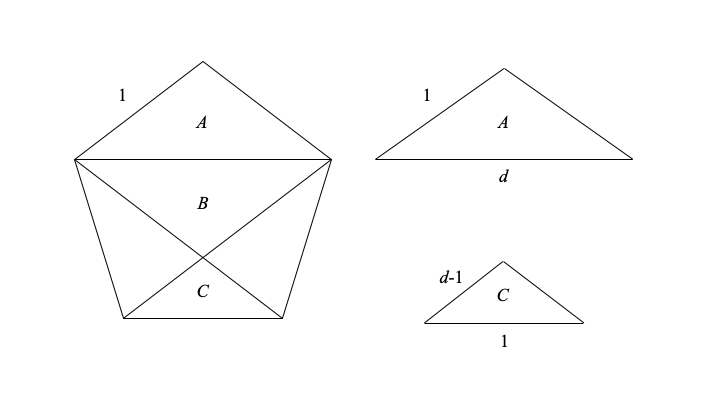
\includegraphics[scale=0.4]{img/pentagram-unit.png}
 \captionsetup{labelformat=empty}
 \caption{边长为1的正五边形}
 \label{fig:pentagram-unit}
\end{figure}

\item 使用$\lambda$变换规则验证$tail\ (cons\ p\ q) = q$。

函数$cons$和$tail$的$\lambda$表达式为:
\[
\begin{array}{rcl}
cons & = & a \mapsto b \mapsto f \mapsto f\ a\ b \\
tail & = & c \mapsto c\ (a \mapsto b \mapsto b)
\end{array}
\]

我们据此来验证$tail\ (cons\ p\ q) = q$这一关系:

\[
\begin{array}{rcl}
tail\ (cons\ p\ q) & = & (c \mapsto c\ (a \mapsto b \mapsto b))\ (cons\ p\ q) \\
                   & \xrightarrow{\beta} & (cons\ p\ q)\ (a \mapsto b \mapsto b) \\
                   & = & ((a \mapsto b \mapsto f \mapsto f\ a\ b)\ p\ q)\ (a \mapsto b \mapsto b) \\
                   & \xrightarrow{\beta} & ((b \mapsto f \mapsto f\ p\ b)\ q)\ (a \mapsto b \mapsto b) \\
                   & \xrightarrow{\beta} & (f \mapsto f \mapsto f\ p\ q)\ (a \mapsto b \mapsto b) \\
                   & \xrightarrow{\beta} & (a \mapsto b \mapsto b)\ p\ q \\
                   & \xrightarrow{\beta} & (b \mapsto b)\ q \\
                   & \xrightarrow{\beta} & q
\end{array}
\]

\item 可以仅仅使用$\lambda$演算来定义自然数。下面是丘奇数的定义:
\[
\begin{array}{r@{\quad:\quad}l}
0 & \lambda f . \lambda x . x \\
1 & \lambda f . \lambda x . f\ x \\
2 & \lambda f . \lambda x . f\ (f\ x) \\
3 & \lambda f . \lambda x . f\ (f\ (f\ x)) \\
  & ...
\end{array}
\]
请利用第一章介绍的内容,定义丘奇数的加法和乘法。

自然数$n$的丘奇数含义是将函数$f$向$x$应用$n$次。我们先定义后继函数:

\[
succ = \lambda n . \lambda f . \lambda x . f\ (n\ f\ x)
\]

其含义是;$f^{n+1}(x)) = f(f^n(x))$。然后定义自然数加法为:

\[
plus = \lambda m . \lambda n . \lambda f . \lambda x . m\ f\ (n\ f\ x)
\]

其含义是:$f^{m + n}(x) = f^m(f^n(x))$。乘法定义为:

\[
mul = \lambda m . \lambda n . \lambda f . \lambda x . m\ (n\ f)\ x
\]

其含义为:$f^{m n} = (f^n)^m(x)$。

\item 以下是丘奇布尔值的定义,以及逻辑运算的一种实现:
\[
\begin{array}{r@{\quad:\quad}l}
\textbf{true} & \lambda x . \lambda y . x \\
\textbf{false} & \lambda x . \lambda y . y \\
\textbf{and} & \lambda p . \lambda q . p\ q\ p \\
\textbf{or} & \lambda p . \lambda q . p\ p\ q \\
\textbf{not} & \lambda p . p\ \textbf{false}\ \textbf{true}
\end{array}
\]
其中\textbf{false}的定义和丘奇数0的定义本质上是相同的。试用$\lambda$变换证明:\textbf{and}\ \textbf{true}\ \textbf{false} = \textbf{false};你能给出if...then...else...语句的$\lambda$定义么?

\blre
and\ true\ false & = & (\lambda p . \lambda q . p\ q\ p)\ true\ false \\
 & \xrightarrow{\beta} & true\ false\ true \\
 & = & (\lambda x . \lambda y . x)\ false\ true \\
 & \xrightarrow{\beta} & false \\
\elre

if ... then ... else ...语句的定义:$\lambda p . \lambda a . \lambda b . p\ a\ b$

\item 不用抽象的叠加操作$foldt$,通过递归定义二叉树的逐一映射$mapt$;

\[ \begin{cases}
mapt(f, nil) & = nil \\
mapt(f, node(l, x, r)) & = node(mapt(f, l), f(x), mapt(f, r)) \\
\end{cases}\]

\item 定义一个函数$depth$,计算一棵二叉树的最大深度;

\[
depth = foldt(one, x, y \mapsto 1 + max(x, y), 0)
\]

其中$one$为常函数,总返回1:$one = x \mapsto 1$。

\item 有人认为,二叉树的抽象叠加操作$foldt$应该这样定义:
\[
\begin{array}{l}
foldt(f, g, c, nil) = c \\
foldt(f, g, c, node(l, x, r)) = foldt(f, g, g(foldt(f, g, c, l), f(x)), r)
\end{array}
\]
也就是说,$g : (B \times B) \to B$是一个类似于加法这样的二元函数。能否利用这个$foldt$定义逐一映射$mapt$?


\item 排序二叉树(又称二叉搜索树)是一种特殊的二叉树,如果二叉树的元素类型A是可比较的,并且对任何非空节点$node(l, k, r)$都满足:左子树$l$中的任何元素都小于$k$,右子树$r$中的任何元素都大于$k$。定义二叉树的插入函数$insert(x, t) : (A \times Tree\ A) \to Tree\ A$

\item 为多叉树定义逐一映射。能否利用多叉树的叠加操作来定义?如果不能,应当怎样修改叠加操作?

\end{enumerate}

\section{群、环、域}

\begin{Exercise}
\Question{全体偶数在加法下是否构成一个群?}
\Question{能否找到一个整数的子集,使得它在整数乘法下构成一个群?}
\Question{所有正实数在乘法下是否构成一个群?}
\Question{整数在减法下是否构成一个群?}
\Question{举一个只有两个元素的群的例子。}
\Question{魔方群的单位元是什么?$F$的逆元是什么?}
\end{Exercise}

\begin{Exercise}
\Question{布尔值构成的集合\{True, False\},在“逻辑或”运算$\lor$下构成一个幺半群。称为任意(Any)逻辑幺半群。它的单位元是什么?}
\Question{布尔值构成的集合\{True, False\},在“逻辑与”运算$\land$下构成一个幺半群。称为全部(All)逻辑幺半群。它的单位元是什么?}
\Question{对可比类型的元素进行比较时,会有三种结果,我们把它们抽象为$\{<, =, >\}$\footnote{一些编程语言,如C、C++、Java用负数、零、正数表示这三种关系。Haskell中用GT, EQ, LE表示。},针对这个集合,定义一个二元运算使得它们构成一个幺半群。这个幺半群的单位元是什么?}
\Question{证明群、幺半群、半群的幂满足交换律:$x^mx^n = x^nx^m$}
\end{Exercise}

\begin{Exercise}
\Question{奇偶判断函数在整数加群$(Z,+)$和布尔逻辑与群$(Bool, \land)$下是否构成同态?去除0元素的整数乘法群呢?}
\Question{假定两个群$G$和$G'$在映射下同态,群$G$中的元$a \to a'$,那么$a$和$a'$的阶是否相同?}
\Question{证明一个变换群的单位元一定是恒等变换。}
\end{Exercise}

\begin{Exercise}
\Question{列出$S_4$的全体元素。}
\Question{将$S_3$的所有元写成不相连的循环置换的乘积。}
\Question{编程将$k$-循环的乘积转换回置换。}
\end{Exercise}

\begin{Exercise}
\Question{证明循环群一定是阿贝尔群。}
\end{Exercise}

\begin{Exercise}
\Question{证明子群的判定定理\ref{theorem:subgroup}。}
\Question{列出图\ref{fig:right-cosets-S3}中$H$的左陪集。}
\end{Exercise}

\begin{Exercise}
\Question{今天是星期日,$2^{100}$天以后是星期几?}
\Question{任给两个串(字符串或者列表),如何通过编程判断它们可以连成相同的项链?}
\Question{编程实现埃拉托斯特尼筛法。}
\Question{利用埃拉托斯特尼筛法的思想,编程产生2到100内正整数的欧拉$\upphi$函数表。}
\Question{编程实现模乘的幂运算,并实现费马素数检测。}
\end{Exercise}

\begin{Exercise}
\Question{证明本节的定理,一个没有零因子的环里,两个消去律成立。}
\Question{证明所有形如$a + b \sqrt{2}$,其中$a, b$是整数的实数对于普通加法和乘法构成一个整环。}
\end{Exercise}

\begin{Exercise}
\Question{证明$Q[a, b] = Q[a][b]$,其中$Q[a, b]$是所有由$a, b$组成的表达式如$2ab, a + a^2b$等。}
\end{Exercise}

\begin{Exercise}
\Question{试证明:对于有理数系数的任何多项式$p(x)$,若$E/Q$是扩域,$f$是$E$上的$Q$-自同构,则有$f(p(x)) = p(f(x))$。}
\Question{考虑复数,多项式$p(x) = x^4-1$的分裂域是什么?它的$Q$-自同构中有哪些变换?}
\Question{尝试写出二次方程$x^2 - bx + c = 0$的伽罗瓦群。}
\Question{证明,如果$p$是素数,则方程$x^p - 1$的伽罗瓦群是$q-1$阶的循环群$C_{q-1}$。}
\end{Exercise}

\begin{Exercise}
\Question{考虑5次方程$x^5 - 1 = 0$,它是根式可解的。它的伽罗瓦群和对应的子群链是什么?}
\end{Exercise}

\section{范畴}

\begin{Exercise}
\Question{证明恒等箭头是唯一的(提示:可以参考上一章中群单位元唯一性的证明)。}
\Question{验证幺半群$(S, \cup, \varnothing)$(群元素是集合,二元运算是集合的并,单位元是空集)和$(N, +, 0)$(群元素是自然数,二元运算是加法,单位元是零)都是只含有一个对象的范畴。}
\Question{第一章中我们介绍了自然数的皮亚诺公理,并且介绍了和皮亚诺算术同构的其它结构,例如链表等。这些完全可以用范畴来解释。这一结论是德国数学家戴德金发现的,尽管当时还没有范畴论。我们今天将这一范畴命名为皮亚诺范畴$\pmb{Pno}$。范畴中的对象为$(A, f, z)$,其中$A$为元素的集合,对于自然数来说这个集合是全体自然数$N$;$f: A \to A$是后继函数,对于自然数来说,就是$succ$;$z \in A$是起始元素,对于自然数来说是0。任给两个皮亚诺对象$(A, f, z)$和$(B, g, c)$,现在定义从$A$到$B$的态射
\[
A \arrowto{\phi} B
\]
它满足

\[
\phi \circ f = g \circ \phi \quad \text{且} \quad \phi(z) = c
\]

试验证$\pmb{Pno}$的确是一个范畴。}
\end{Exercise}

\begin{Exercise}
\Question{请使用叠加操作$foldr$来定义列表函子的箭头映射。}
\Question{证明可能函子和列表函子的组合$\mathbf{Maybe} \circ \mathbf{List}$与$\mathbf{List} \circ \mathbf{Maybe}$仍然是函子。}
\Question{证明任意函子的组合$\mathbf{G} \circ \mathbf{F}$仍然是函子。}
\Question{思考一个预序集范畴上的函子的例子。}
\Question{回顾第二章中介绍的二叉树,请定义一个二叉树函子。}
\end{Exercise}

\begin{Exercise}
\Question{考虑偏序集(poset)中的两个对象,它们的积是什么?余积是什么?}
%\Question{考虑集合范畴$\pmb{Set}$,积中的两个箭头$fst, snd$是右消去(epic)的么?余积中的两个箭头$left, right$是左消去(monic)的么?}
\Question{证明余积的吸收率,并验证余积函子的组合性质。}
\end{Exercise}

\begin{Exercise}
\Question{证明$swap$满足自然变换的条件$(g \times f) \circ swap = swap \circ (f \times g)$}
\Question{证明多态函数$length$是一个自然变换,其定义如下:
\[
\begin{array}{l}
length : [A] \to Int \\
length\ [] = 0 \\
length\ (x:xs) = 1 + length\ xs
\end{array}
\]
}
\Question{自然变换也可以进行组合,考虑两个自然变换$\mathbf{F} \arrowto{\phi} \mathbf{G}$和$\mathbf{G} \arrowto{\psi} \mathbf{H}$,对于任意箭头$A \arrowto{f} B$,试画出自然变换组合$\phi \circ \psi$的范畴图,并列出可交换性的条件。}
\end{Exercise}

\begin{Exercise}
\Question{在本节的例子中,我们说在一个偏序集中,如果存在最小值(或最大值),则最小值(或最大值)就是起始对象(或终止对象)。考虑全体偏序集构成的范畴$\pmb{Poset}$,如果存在起始对象,它是什么?如果存在终止对象,它是什么?}
\Question{皮亚诺范畴$\pmb{Pno}$(参见本章第一节的习题2)中,什么样的对象$(A, f, z)$是起始对象?终止对象是什么?}
\end{Exercise}

\begin{Exercise}
\Question{验证$\pmb{Exp}$的确是一个范畴,指出$id$箭头和箭头的组合。}
\Question{反射律$curray\ apply = id$中,$id$的下标是什么?请用另一种方法证明它。}
\Question{我们称下面的等式
\[
(curry\ f) \circ g = curry(f \circ (g \times id))
\]
为克里化的融合律。请画出它的范畴图并证明它。}
\end{Exercise}

\begin{Exercise}
\Question{画出群的可逆性公理的范畴图。}
\Question{$p$是一个素数,使用群的F-代数,为整数模$p$乘法群(可以参考上一章)定义一个$\alpha$箭头。}
\Question{参考上一章环的定义,定义环的F-代数。}
\Question{F-代数范畴上的$id$箭头是什么?箭头组合是什么?}
\end{Exercise}

\begin{Exercise}
\Question{可否把类自然数函子写成如下递归的形式?谈谈你的看法。
\begin{lstlisting}
data NatF A = ZeroF | SuccF (NatF A)
\end{lstlisting}
}
\Question{我们可以为$\mathbf{NatF} Int \to Int$定义一个$\alpha$箭头,名叫$eval$:
\[
\begin{array}{l}
eval : \mathbf{NatF} Int \to Int \\
eval\ ZeroF = 0 \\
eval\ (SuccF\ n) = n + 1 \\
\end{array}
\]
如果迭代地将$A' = \mathbf{NatF} A$代入$\mathbf{NatF}$函子$n$次。我们把这样得到的函子记为$\mathbf{NatF}^n A$。试思考能否定义下面的$\alpha$箭头:
\[
\begin{array}{l}
eval : \mathbf{NatF}^n Int \to Int \\
\end{array}
\]
}
\end{Exercise}

\begin{Exercise}
\Question{对二叉树函子$\mathbf{TreeF}\ A\ B$,固定$A$,利用不动点验证$(\mathbf{Tree}\ A, [nil, branch])$是初始代数。}
\end{Exercise}

\section{推导}
\begin{Exercise}
\Question{验证从左侧叠加也可以表示为$foldr$:
\[
foldl\ f\ z\ xs = foldr\ (b\ g\ a \mapsto g\ (f\ a\ b))\ id\ xs\ z
\]}
\Question{证明以下列表的构建——叠加形式:
\[
\begin{array}{l}
concat\ xss = build\ (f\ z \mapsto foldr\ (xs\ x \mapsto foldr\ f\ x xs)\ xss) \\
map\ f\ xs = build\ (\oplus\ z \mapsto foldr\ (y\ ys \mapsto (f\ y) \oplus ys)\ z\ xs) \\
filter\ f\ xs = build\ (\oplus\ z \mapsto foldr\ (x\ xs' \mapsto
  \begin{cases}
     f(x): & x \oplus xs' \\
    \text{否则}: & xs' \\
  \end{cases})\ z\ xs) \\
repeat\ x = build\ (\oplus\ z \mapsto let\ r = x \oplus r\ in\ r) \\
\end{array}
\]
}
\Question{利用融合律化简快速排序算法:
\[
\begin{cases}
qsort\ [] = [] \\
qsort\ (x:xs) = qsort\ [a | a \in xs, a \leq x] \doubleplus [x] \doubleplus qsort\ [a | a \in xs, x < a] \\
\end{cases}\]
提示:将ZF表达式\footnote{全称为“策梅罗——弗兰克尔表达式”。指集合论中$\{f(x) | x \in X, p(x), q(x), ...\}$这样的集合构建表达式。我们在下一章介绍无穷和集合论时会再次遇到它。}转换为$filter$。}
\Question{利用范畴论验证融合律的类型限制。提示:考虑向下态射的类型。}
\end{Exercise}

\begin{Exercise}
\Question{利用融合律化简算式求值的定义$eval = sum \circ map\ (product \circ (map\ dec))$。}
\Question{如何从左侧扩展出所有的算式?}
\Question{下面定义可以将算式翻译为字符串:
\[
str = (join\ \text{``+''}) \circ (map\ ((join\ \text{``} \times \text{''}) \circ (map\ (show \circ dec))))
\]
其中$show$可以将数字转换为字符串。函数 $join(c, s)$ 将一组字符串$s$用$c$连接起来,例如 $join($``\#''$, [$``abc'', ``def''$]) = $``abc\#def'' 。利用融合律化简$str$的定义。
}
\end{Exercise}


\section{无穷}

\begin{Exercise}
\Question{第一章中,我们用叠加操作实现了斐波那契数列,如何用$iterate$定义斐波那契数列潜无穷?}
\Question{用叠加操作定义$iterate$。}
\end{Exercise}

\begin{Exercise}
\Question{利用第四章中介绍的不动点定义,证明$Stream$是$StreamF$的不动点。}
\Question{试定义反折叠$unfold$}
\end{Exercise}

\begin{enumerate}
\item 数论中的算术基本定理说:任何一个大于1的整数都可以唯一地表示成若干素数的乘积。有一道编程趣题,要求判断一段文字$T$中,是否包含一个字符串$W$的某种排列。试利用算术基本定理,和素数流解决这道题目。

我们的思路是,将每一个不同字符对应到一个素数上去,a对应2,b对应3,c对应5……。这样任意给定一个字符串$W$,不管它是否包含重复的字符,我们都可以把它表示为素数的乘积:

\[
F = \prod p_c , c \in W
\]

我们称其为字符串$W$的数论指纹$F$。如果$W$是空串,我们规定它的指纹等于1。根据整数乘法的交换律,我们知道无论$W$怎样排列,其数论指纹都不变,并且根据算术基本定理,这个数论指纹是唯一的。现在我们就得到了一个特别简洁的解法:我们首先计算出$W$的数论指纹$F$,然后用一个长度为$|W|$的窗口沿着$T$从左向右滑动。一开始我们需要计算$T$在这个窗口内的数论指纹,并和$F$比较,如果相等就说明$T$包含$W$的某种排列。如果不等我们将这个窗口向右滑动一个字符。此时我们可以非常容易地计算新窗口内的数论指纹:只要把滑出的字符对应的素数除掉,再把滑入的字符对应的素数乘上就可以了。任何时候如果新窗口内的数论指纹等于$F$,就说明找到了一个排列。当然为了获得每个不同字符对应的素数,我们还要利用埃拉托斯特尼筛法产生一串素数。下面是一段示例算法:

\begin{algorithmic}
\Function{contains?}{$W, T$}
  \State $P \gets ana \ era \ [2, 3, ...]$ \Comment{素数序列}
  \If{$W = \phi$}
    \State \Return True
  \EndIf
  \If{$|T| < |W|$}
    \State \Return False
  \EndIf
  \State $\displaystyle m \gets \prod P_c, c \in W$
  \State $\displaystyle m' \gets \prod P_c, c \in T[1...|W|]$
  \For{$i \gets |W| + 1$ to $|T|$}
    \If{$m = m'$}
      \State \Return True
    \EndIf
    \State $m' \gets m' \times P_{T_i} / P_{T_{i - |W|}} $
  \EndFor
  \State \Return $m = m'$
\EndFunction
\end{algorithmic}

\end{enumerate}

\begin{Exercise}
\Question{我们用图\ref{fig:NNtoN}建立了房间和任意旅游团的客人间的一一映射。第$i$号旅游团的第$j$号客人应该入住几号房间?第$k$个房间里住了哪号旅游团的哪位客人?}
\Question{希尔伯特旅馆第三天的故事的解法并不唯一,图\ref{fig:PWW-NNtoN}是《无需语言的证明》一书的封面。试根据此图给出另一种编号方案?
%% \begin{figure}[htbp]
%%  \centering
%%  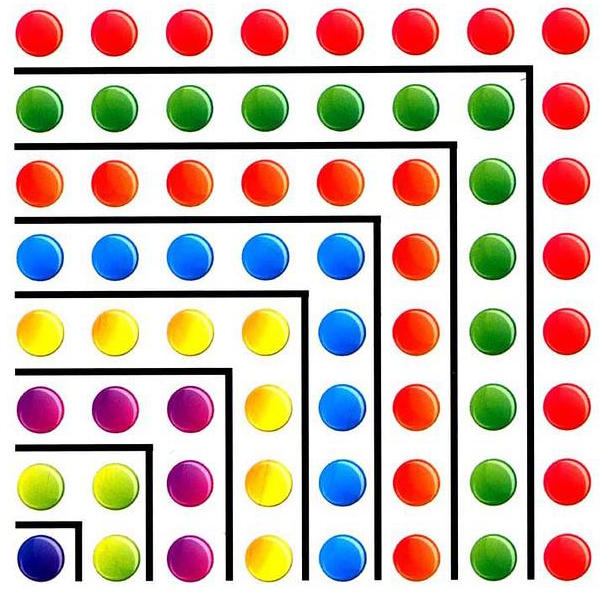
\includegraphics[scale=0.2]{img/PWW.eps}
%%  \caption{《无需语言的证明》封面局部}
%%  \label{fig:PWW-NNtoN}
%% \end{figure}
}
\end{Exercise}

\begin{Exercise}
\Question{令$x = 0.9999....$, 则$10x = 9.9999...$,做减法得$10x - x = 9$,解方程得$x = 1$。因此得到结论$1 = 0.9999...$。这一证明正确么?}
\end{Exercise}

\begin{Exercise}
\Question{在两个镜子中间点燃一支蜡烛,你看到了什么?这是潜无穷还是实无穷?}
\end{Exercise}

\section{悖论}

\begin{Exercise}
\Question{我们可以用语言定义数,例如“最大的两位数”定义了99。定义一个集合,是所有不能用20个以内的字描述的数字。考虑这样一个元素:“不能用20个以内的字描述的最小数”,它是否属于这个集合?}
\Question{“这个世界上唯一不变的是变化”——这句话是否是罗素悖论?}
\Question{本章开头苏格拉底的话是否是罗素悖论?}
\end{Exercise}

\begin{Exercise}
\Question{尝试给出费马大定理的印符串。}
\Question{尝试用印符推理规则证明加法结合律。}
\end{Exercise}

\begin{Exercise}
\Question{利用新加入的归纳规则证明$\forall a: (0 + a) = a$}
\end{Exercise}

\ifx\wholebook\relax \else
\begin{thebibliography}{99}

\bibitem{Lockhart2012}
[美] 保罗$\cdot$洛克哈特 著, 王凌云 译. ``度量——一首献给数学的情歌''. 人民邮电出版社. 2015, ISBN: 9787115393180

\end{thebibliography}

\expandafter\enddocument
%\end{document}

\fi
